\documentclass[10pt,aspectratio=169]{beamer}

\usepackage{amsmath,amssymb}
\usepackage{mathtools}
\usepackage{booktabs}
\usepackage{graphicx}
\usepackage{tikz}
\usetikzlibrary{positioning,arrows.meta}

\graphicspath{{../figures/}}

\usetheme{metropolis}                  % falls back gracefully if unavailable
\setbeamertemplate{caption}{\insertcaption}
\setbeamerfont{caption}{size=\scriptsize}

\newcommand{\sigmoid}{\sigma}
\newcommand{\diag}{\operatorname{diag}}
\newcommand{\rel}{\mathrm{REL}}
\newcommand{\res}{\mathrm{RES}}
\newcommand{\unc}{\mathrm{UNC}}
\newcommand{\bs}{\mathrm{BS}}

\title{Predicting NBA Game Winners}
\subtitle{Logistic regression, ELO, calibration, and the road to beating the market}
\author{Angel \and Mehmet Can \and Andrew}
\institute{Math 17 --- Mathematics for Machine Learning}
\date{}

\begin{document}

% ----------------------------------------------------------------------
\begin{frame}
  \titlepage
\end{frame}

% ----------------------------------------------------------------------
\begin{frame}{What we want to do}
  \begin{itemize}
    \item Given a scheduled NBA game, estimate
      $p = \Pr(\text{home wins} \mid \text{features})$.
    \item Build the entire mathematical pipeline from first principles:
      likelihood $\to$ loss $\to$ gradient $\to$ Hessian $\to$
      optimiser $\to$ metric.
    \item Evaluate on the held-out 20\% of the 2023--24 and 2024--25
      seasons (528 real NBA games).
    \item Long-term goal: out-predict the prediction-market crowd on log-loss.
  \end{itemize}

  \vfill
  \textbf{Headline result.} L2-regularised logistic regression: \textbf{67.2\%
  accuracy, log-loss 0.595, AUC 0.740} on a strict chronological hold-out.
\end{frame}

% ----------------------------------------------------------------------
\begin{frame}{The data}
  \textbf{Source:} \texttt{basketball-reference.com} game schedules
  (regular season + playoffs).
  \begin{itemize}
    \item 2{,}640 games over 2023--24 and 2024--25
    \item All 30 NBA franchises
    \item Home win rate 54.6\%
    \item Chronological 80/20 split: 2{,}112 train, 528 test
  \end{itemize}

  \textbf{Features used by the LR (10 columns):}
  \begin{itemize}
    \item Rolling 10-game differentials of offensive / defensive / net
      ratings, pace, scoring margin, and win percentage
    \item Rest-day differential, back-to-back flags
    \item ELO logit (link to next slide)
  \end{itemize}

  \emph{All rolling features are shifted by one game} to prevent
  look-ahead leakage; standardisation is fit on the training rows
  only.
\end{frame}

% ----------------------------------------------------------------------
\begin{frame}{The math: from Bernoulli MLE to BCE}
  \[
    p_i = \sigmoid(x_i^\top w + b), \qquad \sigmoid(z) = \tfrac{1}{1 + e^{-z}}.
  \]
  Bernoulli likelihood
  $\mathcal{L} = \prod p_i^{y_i}(1-p_i)^{1-y_i}$ $\;\Longrightarrow\;$
  \alert{binary cross-entropy}:
  \[
    J(w,b) = -\frac{1}{n}\sum_i \bigl[y_i \log p_i + (1-y_i)\log(1-p_i)\bigr].
  \]

  Gaussian prior on the weights $\Longrightarrow$ L2 penalty
  ($\lambda = 1/(n\sigma^2)$):
  \[
    J_\lambda(w,b) \;=\; J(w,b) + \tfrac{\lambda}{2}\lVert w\rVert_2^2.
  \]

  \vfill
  \textbf{The loss is not arbitrary.} It is the negative log-likelihood
  under the model, and L2 is the MAP shift under a Gaussian prior.
\end{frame}

% ----------------------------------------------------------------------
\begin{frame}{Gradient, Hessian, convexity}
  With $p = \sigmoid(Xw + b\mathbf{1})$:
  \begin{align*}
    \nabla_w J_\lambda &= \tfrac{1}{n} X^\top(p - y) + \lambda w\\
    H_{ww} &= \tfrac{1}{n} X^\top \diag(p \odot (1-p)) X + \lambda I.
  \end{align*}

  $p_i(1-p_i) > 0$, so $X^\top \diag(\cdot) X$ is PSD; with $\lambda > 0$
  the Hessian is positive definite. Hence
  \[
    \boxed{\,J_\lambda \text{ is strictly convex with a unique minimiser.\,}}
  \]

  \pause
  \vfill
  \textbf{Why we care.} If every optimiser converges, they converge to
  the \emph{same} answer. Speed is the only thing that differs.
\end{frame}

% ----------------------------------------------------------------------
\begin{frame}{Three optimisers, one minimum}
  \begin{center}
    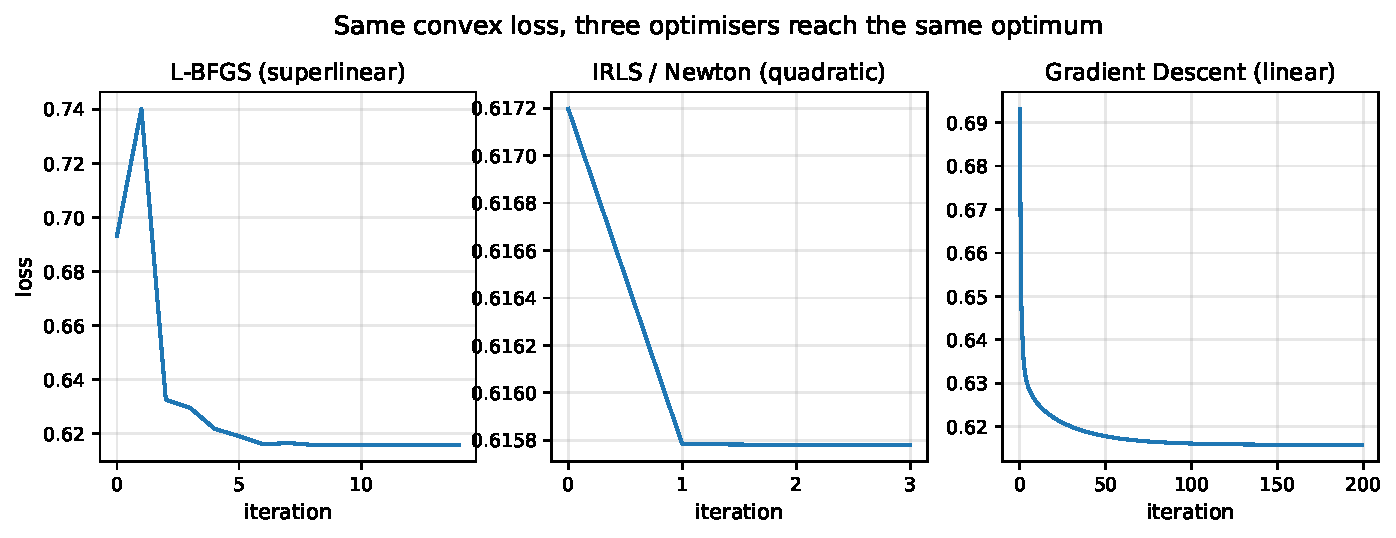
\includegraphics[width=\linewidth]{loss_curves.pdf}
  \end{center}
  \begin{itemize}
    \item \textbf{L-BFGS} (default): quasi-Newton, superlinear, $O(nd)$/step.
    \item \textbf{IRLS = Newton}: solves a weighted ridge regression each step;
      quadratic convergence, $O(nd^2 + d^3)$/step.
    \item \textbf{Gradient descent}: linear convergence, $O(nd)$/step.
  \end{itemize}
\end{frame}

% ----------------------------------------------------------------------
\begin{frame}{ELO is logistic regression}
  Define $\Pr(A \text{ beats } B) = \sigmoid((R_A - R_B)/s)$ with
  $s = 400/\ln 10$. \\
  This is identical to $1/(1 + 10^{-(R_A - R_B)/400})$.

  \alert{So ELO is logistic regression with one feature (the rating
  difference) and a known scale.}

  \pause\vfill
  \textbf{ELO updates = SGD on log-loss.} For one game
  $\partial L/\partial R_A = (p - y)/s$, $\partial L/\partial R_B = -(p - y)/s$. One SGD step with
  rate $Ks$:
  \[
    R_A \leftarrow R_A + K(y - p), \qquad
    R_B \leftarrow R_B - K(y - p).
  \]
  The K-factor is the SGD learning rate.
\end{frame}

% ----------------------------------------------------------------------
\begin{frame}{ELO on real data (sanity check)}
  \begin{center}
    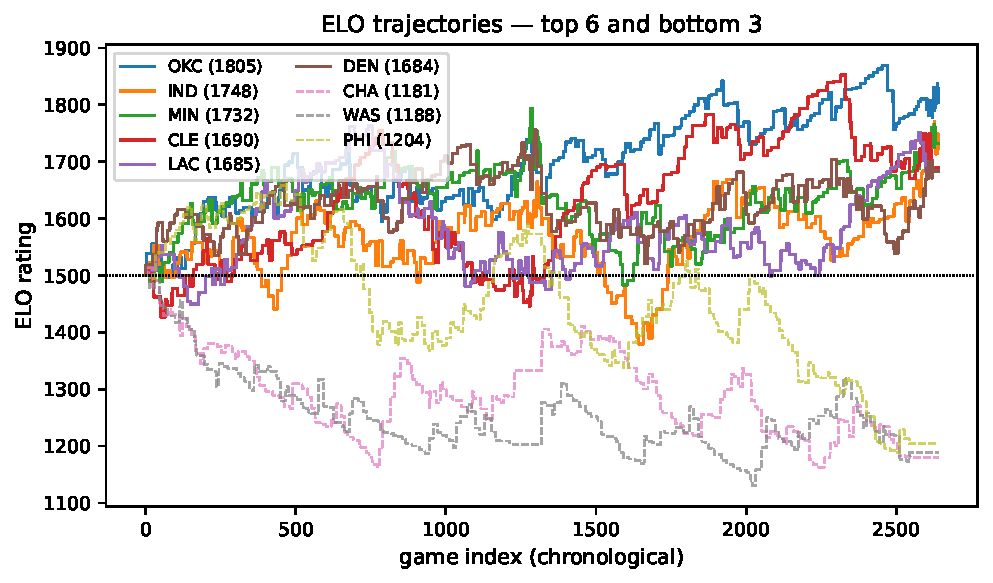
\includegraphics[width=0.85\linewidth]{elo_trace.pdf}
  \end{center}
  Oklahoma City finishes at 1805 (real-world 2024--25 champions);
  Charlotte / Washington / Philadelphia at the bottom matches their
  records. The two visible compressions are end-of-season mean
  reversion.
\end{frame}

% ----------------------------------------------------------------------
\begin{frame}{Adding teams as learned vectors --- the NN}
  \begin{columns}[t]
    \column{0.55\textwidth}
    \begin{itemize}
      \item For each team $t$, learn a vector $e_t \in \mathbb{R}^k$.
      \item Concatenate $[x;\, e_h - e_a]$ (\emph{difference} keeps the
        model invariant under team relabelling --- same idea as ELO).
      \item One ReLU hidden layer, sigmoid head.
      \item Loss: BCE + L2 on weights + separate L2 on embeddings
        (Gaussian prior on team strength).
      \item Optimiser: Adam, early stopping on val.
    \end{itemize}

    \column{0.45\textwidth}
    \scriptsize
    \[
      \begin{aligned}
        u   &= [x;\, e_h - e_a] \\
        h_1 &= \mathrm{ReLU}(W_1 u + b_1) \\
        z   &= w_2^\top h_1 + b_2 \\
        p   &= \sigmoid(z)
      \end{aligned}
    \]
    \vskip 1em
    \emph{Backprop derivation in full in the module docstring; verified
    by a finite-difference test.}
  \end{columns}
\end{frame}

% ----------------------------------------------------------------------
\begin{frame}{Metrics from first principles}
  Implemented from scratch in numpy; cross-checked against sklearn in
  tests.

  \begin{itemize}
    \item \textbf{Log-loss} (same formula as training loss) --- a
      proper scoring rule.
    \item \textbf{Brier} $\bs = (1/n)\sum (p_i - y_i)^2$
      with Murphy's three-way decomposition:
      \[
        \bs = \rel - \res + \unc.
      \]
      \begin{itemize}\scriptsize
        \item $\rel$ --- bin-wise calibration error (lower is better)
        \item $\res$ --- skill: how much bin frequencies deviate from $\bar y$
        \item $\unc = \bar y(1 - \bar y)$ --- irreducible label variance
      \end{itemize}
    \item \textbf{AUC} via Mann--Whitney U with proper tie handling.
    \item \textbf{ECE} --- weighted gap between bin means and bin
      frequencies.
  \end{itemize}
\end{frame}

% ----------------------------------------------------------------------
\begin{frame}{Calibration (post-hoc)}
  A model can have high AUC and still be miscalibrated. Two methods:

  \textbf{Platt scaling.} Fit a 1-D LR on the model's logits:
  $P(Y=1 | z) = \sigmoid(A z + B)$. \\
  With Platt smoothing on the targets to avoid overfit on small
  calibration sets.

  \textbf{Isotonic regression.} Best non-decreasing step function
  $g$ minimising $\sum w_i (g_i - y_i)^2$. Implemented with
  \emph{pool-adjacent-violators} in $O(n)$.

  \begin{center}
    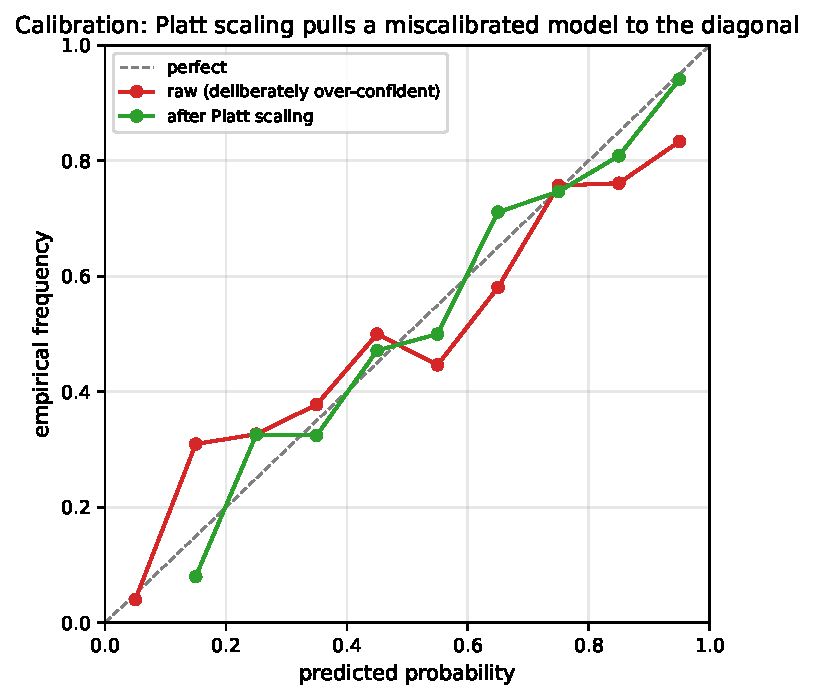
\includegraphics[width=0.65\linewidth]{calibration_demo.pdf}
  \end{center}
\end{frame}

% ----------------------------------------------------------------------
\begin{frame}{Results --- held-out 20\% (528 games)}
  \centering
  \begin{tabular}{lrrrrr}
    \toprule
    Model        & Acc.   & Log-loss          & Brier           & AUC          & ECE \\
    \midrule
    ELO          & 0.659  & 0.616             & 0.212           & 0.734        & 0.077 \\
    LR (L-BFGS)  & 0.672  & \textbf{0.595}    & \textbf{0.205}  & \textbf{0.740} & 0.044 \\
    LR + Platt   & 0.672  & 0.595             & 0.205           & 0.740        & 0.046 \\
    NN (Adam)    & 0.672  & 0.602             & 0.207           & 0.734        & 0.041 \\
    NN + Platt   & \textbf{0.676}  & 0.601    & 0.207           & 0.734        & \textbf{0.040} \\
    \bottomrule
  \end{tabular}

  \vfill
  \begin{itemize}
    \item LR wins on log-loss, Brier, and AUC.
    \item NN matches accuracy but doesn't reduce log-loss (small
      training sample).
    \item ELO is a strong, free baseline.
    \item LR's resolution $\res = 0.045$, uncertainty $\unc = 0.248$
      $\Rightarrow$ model explains $\sim$18\% of label variance.
  \end{itemize}
\end{frame}

% ----------------------------------------------------------------------
\begin{frame}{Calibration on real data}
  \begin{center}
    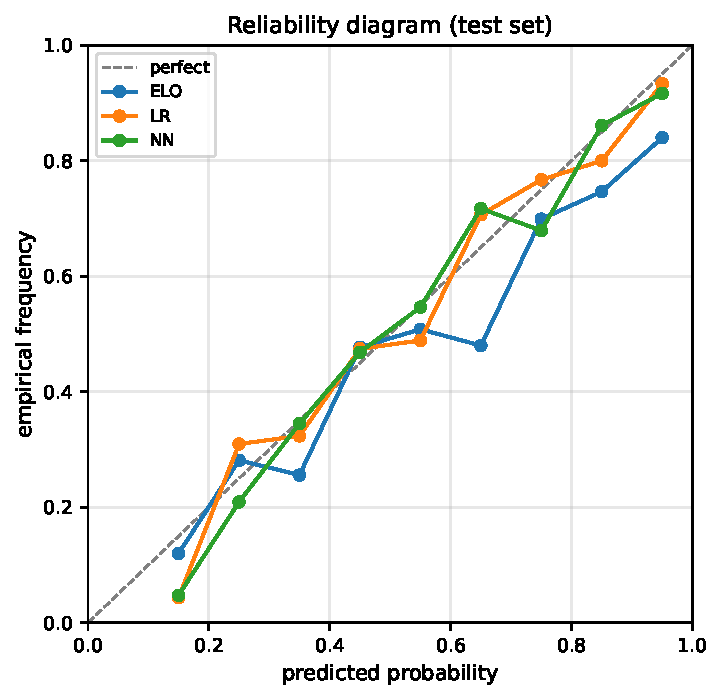
\includegraphics[width=0.55\linewidth]{reliability_combined.pdf}
  \end{center}
  All three models track the diagonal well above $p > 0.4$;
  ELO is mildly over-confident on low-probability home teams. This is
  the geometric picture corresponding to the $\rel$ column in the
  results table.
\end{frame}

% ----------------------------------------------------------------------
\begin{frame}{Side-by-side metrics}
  \begin{center}
    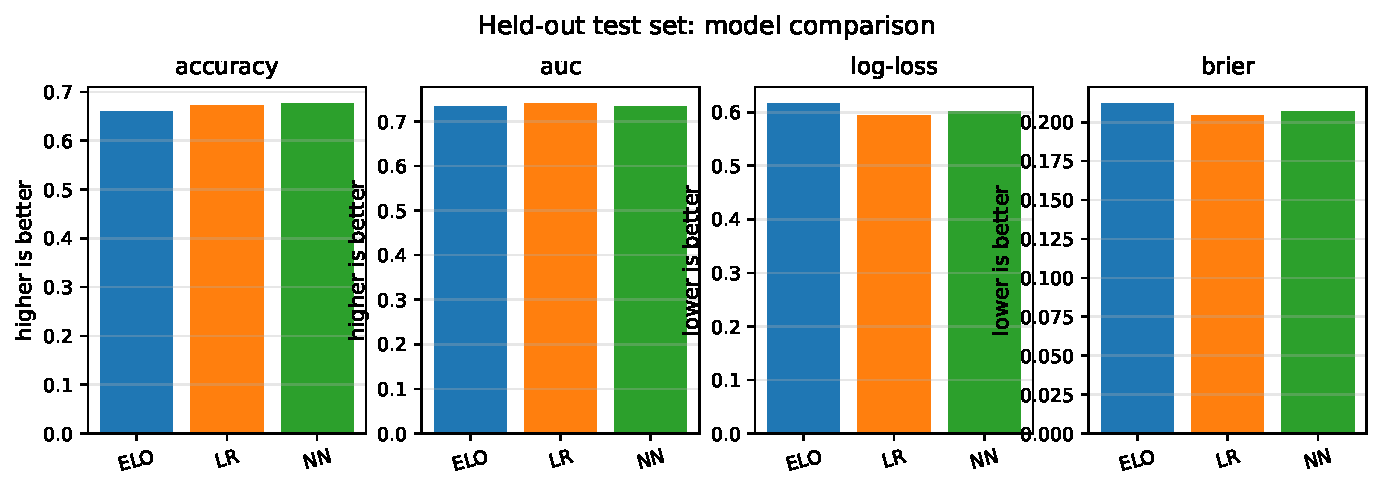
\includegraphics[width=0.9\linewidth]{model_comparison.pdf}
  \end{center}
\end{frame}

% ----------------------------------------------------------------------
\begin{frame}{What's next}
  \begin{enumerate}
    \item \textbf{Market comparison.} Code for devigging Kalshi /
      Polymarket prices, log-loss against the market, and a Kelly
      backtest is already implemented and tested. We need licensed
      historical-odds data to evaluate on the same chronological hold-out.
    \item \textbf{Richer features.} Four-factor counting stats,
      player availability, road-trip schedule features. The data
      adapters are stubbed in; the model code accepts them
      unchanged.
    \item \textbf{In-game model.} Same architecture, with score
      differential and seconds remaining; very similar code path.
  \end{enumerate}
\end{frame}

% ----------------------------------------------------------------------
\begin{frame}{Limitations / honesty}
  \begin{itemize}
    \item Only two seasons of data --- $\sim$2{,}100 training rows.
      Deep models cannot win here.
    \item Without box-score four-factor stats, our offensive / defensive
      ratings are coarse (we use a 100-possession proxy).
    \item Recent NBA home-court advantage has fallen; the model
      learns this from data but it makes the baseline weaker than
      historical literature would suggest.
    \item Beating the market on log-loss may genuinely be infeasible
      on this sample; we will report whatever we find.
  \end{itemize}
\end{frame}

% ----------------------------------------------------------------------
\begin{frame}{Repository}
  \centering
  \texttt{github.com/mehmet-can-yilmaz/nba-predictions}

  \vfill
  \begin{itemize}
    \item Math derivations: \texttt{MATH.md}
    \item Solver implementations: \texttt{src/.../logistic\_regression.py},
      \texttt{elo.py}, \texttt{neural\_net.py}
    \item Metrics + calibration: \texttt{metrics.py}, \texttt{calibration.py}
    \item Market + Kelly: \texttt{market.py}
    \item 30 unit tests pass, including a finite-difference gradient
      check and a cross-check against scikit-learn.
  \end{itemize}

  \vfill
  \begin{center}
    \large \emph{Thank you. Questions?}
  \end{center}
\end{frame}

\end{document}
